\chapter{نتایج و مقایسه} \label{ch:results}
در این فصل نتایج آزمایش‌های کیفی و کمی انجام‌شده با روش پیشنهاد شده برای تقطیع تصاویر خواهد آمد و نتایج کمی با تعدادی از الگوریتم‌های رایج در این حوزه مورد مقایسه قرار می‌گیرند.

\section{ارزیابی کیفی}
ابتدا به صورت بصری به بررسی نتایج روی مجموعه داده برکلی می‌پردازیم.
شکل
\ref{fig.testlambda}
نتایج تقطیع را با سه مقدار مختلف این پارامتر نمایش می‌دهد.
نتایج تقطیع به صورت "تصویر مصنوعی" نمایش داده شده‌اند.
در این تصاویر، به منظور نمایش بهتر قطعات، هر قطعه با رنگ متوسط پیکسل‌های موجود در آن پر شده است.
مشاهده می‌کنیم که برای مقادیر کوچک پارامتر
$\lambda$
قطعات کمتر با یکدیگر ادغام می‌شوند و بسیاری از ابرپیکسل‌های اولیه بدون تغییر باقی می‌مانند.
اما با افزایش مقدار پارامتر
$\lambda$،
ادغام‌های بیشتری صورت گرفته و اندازه قطعات بزرگ‌تر می‌شود.
با توجه به این که در محاسبه طول کد مربوط به هر قطعه،
$\lambda$
ضریب جمله نمایانگر طول کد مورد نیاز برای بازنمایی پارامترهای مدل است، این امر قابل پیش‌بینی بود،
زیرا این طول کد به ازای هر قطعه، به مجموع طول کد افزوده می‌شود و 
بنابراین ضریب بزرگ برای آن همراه با تعداد قطعات زیاد، طول کد کل را بیشتر از حالتی می‌کند که قطعات بزرگ با درست‌نمایی پایین‌تر داشته باشیم.




\begin{figure}[tp]
	\makebox[\linewidth][c]{%
		\begin{subfigure}[b]{.5\textwidth}
			\centering
			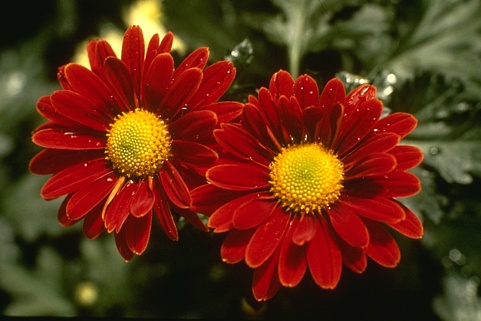
\includegraphics[width=.95\textwidth]{testlambda/original}
			\caption{تصویر اصلی}
		\end{subfigure}%
		\begin{subfigure}[b]{.5\textwidth}
			\centering
			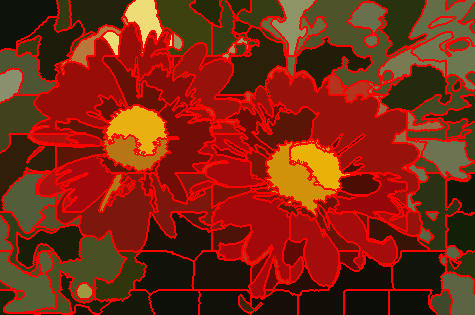
\includegraphics[width=.95\textwidth]{testlambda/10}
			\caption{$\lambda=10$}
		\end{subfigure}%
	}\\[20pt]
	\makebox[\linewidth][c]{%
		\begin{subfigure}[b]{.5\textwidth}
			\centering
			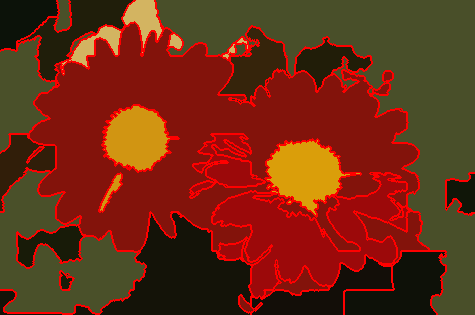
\includegraphics[width=.95\textwidth]{testlambda/100}
			\caption{$\lambda=100$}
		\end{subfigure}%
		\begin{subfigure}[b]{.5\textwidth}
			\centering
			
\includegraphics[width=.95\textwidth]{testlambda/1000}
			\caption{$\lambda=1000$}
		\end{subfigure}%
	}
	\caption{
مقایسه تاثیر مقادیر مختلف پارامتر
$\lambda$
بر کیفیت تقطیع
		\label{fig.testlambda}
	}
\end{figure}





به منظور بررسی بهتر مراحل اجرای الگوریتم،
نتایج اجرای الگوریتم روی دو نمونه از تصاویر مجموعه برکلی در شکل
\ref{fig.sampleOutputs}
آمده است.
شکل‌های ردیف بالا تصاویر اصلی و
شکل‌های ردیف دوم، ابرپیکسل‌های استخراج شده از آن‌ها را نمایش می‌دهند.
پارامترهای الگوریتم SLIC را به گونه‌ای تنظیم نموده‌ایم که به طور تقریبی تعداد 100 ابرپیکسل استخراج شود.
شکل‌های ردیف سوم، نتایج نهایی اجرای الگوریتم پیشنهادی را نمایش می‌دهند و در ردیف آخر، به منظور نمایش بهتر قطعات، تصاویر مصنوعی ساخته شده توسط آن‌ها آمده است.
برای کسب این نتایج، پارامتر
$\lambda$
برابر 100 در نظر گرفته شده است.
استخراج بردارهای ویژگی با پنجره‌های
7$\times$7
انجام شده و مولفه‌ی DC بردارها حذف گردیده است.
مدل آمیخته برازش شده به داده‌های هر قطعه از تصویر، دارای پنج جزء با توزیع vMF بوده و پارامترهای آن پس از مقداردهی اولیه با الگوریتم
\lr{k-means++}،
با روش EM تخمین زده شده است.


\begin{figure}[!tp]
	\makebox[\linewidth][c]{%
		\begin{subfigure}[b]{.5\textwidth}
			\centering
			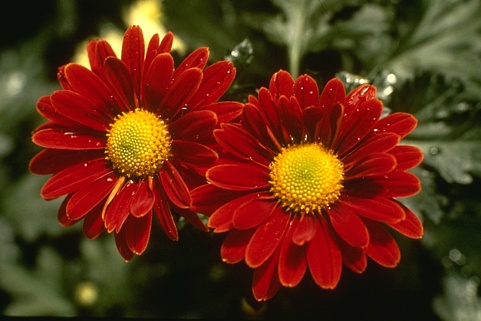
\includegraphics[width=.95\textwidth]{first/124084}
			%\caption{}
		\end{subfigure}%
		\begin{subfigure}[b]{.5\textwidth}
			\centering
			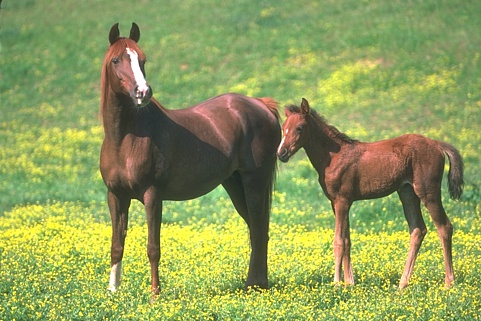
\includegraphics[width=.95\textwidth]{first/113016}
			%\caption{}
		\end{subfigure}%
	}\\
	\makebox[\linewidth][c]{%
		\begin{subfigure}[b]{.5\textwidth}
			\centering
			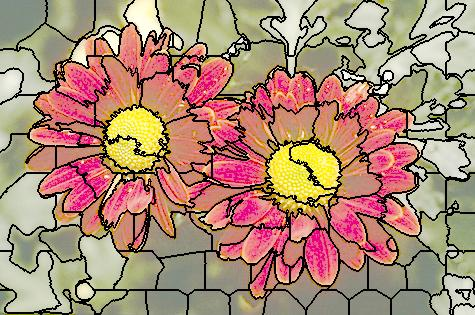
\includegraphics[width=.95\textwidth]{first/124084-sp}
			%\caption{}
		\end{subfigure}%
		\begin{subfigure}[b]{.5\textwidth}
			\centering
			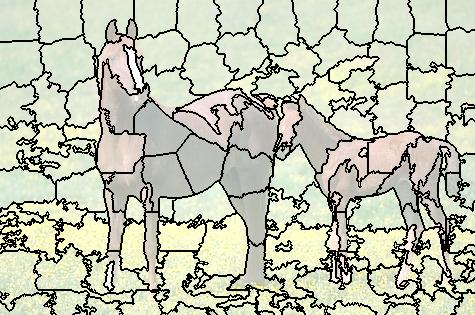
\includegraphics[width=.95\textwidth]{first/113016-sp}
			%\caption{}
		\end{subfigure}%
	}\\
	\makebox[\linewidth][c]{%
		\begin{subfigure}[b]{.5\textwidth}
			\centering
			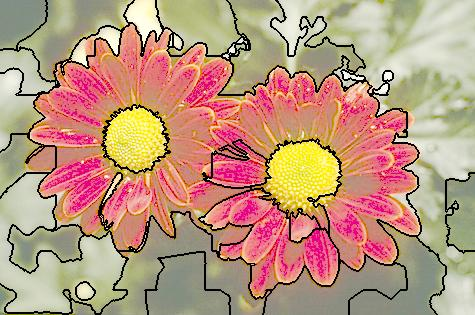
\includegraphics[width=.95\textwidth]{first/124084-result}
%			\caption{}
		\end{subfigure}%
		\begin{subfigure}[b]{.5\textwidth}
			\centering
			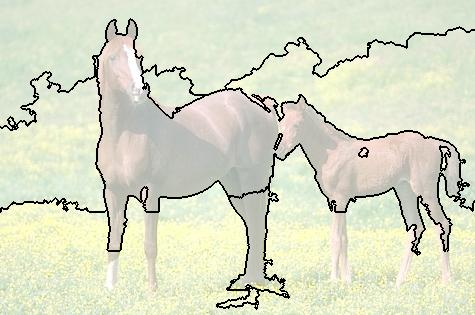
\includegraphics[width=.95\textwidth]{first/113016-result}
%			\caption{}
		\end{subfigure}%
	}\\
	\makebox[\linewidth][c]{%
		\begin{subfigure}[b]{.5\textwidth}
			\centering
			
\includegraphics[width=.95\textwidth]{first/124084-synthetic}
			%\caption{}
		\end{subfigure}%
		\begin{subfigure}[b]{.5\textwidth}
			\centering
			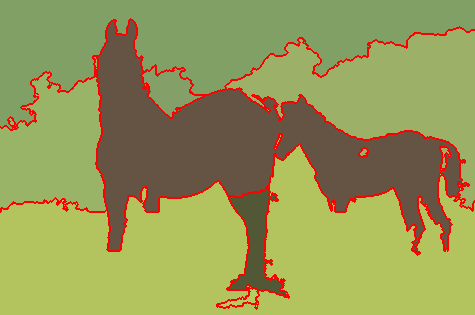
\includegraphics[width=.95\textwidth]{first/113016-synthetic}
			%\caption{}
		\end{subfigure}%
	}
\caption[
نمونه نتایج الگوریتم پیشنهادی روی دو تصویر نمونه
]{
نمونه نتایج الگوریتم پیشنهادی روی دو تصویر نمونه - به ازای هر تصویر (ردیف بالا)، ابرپیکسل‌های استخراج شده با تعداد تقریبی 100 ابرپیکسل (ردیف دوم) و نتیجه نهایی پس از ادغام ابرپیکسل‌ها با پارامتر
$\lambda=100$
(ردیف سوم و چهارم) آمده است.
در ردیف چهارم برای نمایش بهتر، تصاویر مصنوعی حاصل از پر کردن هر قطعه با رنگ متوسط پیکسل‌های موجود در آن آمده است.
\label{fig.sampleOutputs}
}
\end{figure}






محاسبه شده است.

\begin{table}[bh]
	\caption[بررسی مقادیر بهبود طول کد در ادغام قطعات]
	{
بررسی مقادیر بهبود طول کد در ادغام قطعات.
مقادیر بر حسب میلیون واحد اطلاعاتی مبتنی بر لگاریتم طبیعی
(\lr{nat})
هستند.
	}
	\phantomsection
	\label{table.improvement_comparison}
	\begin{center}
		{\setlength{\extrarowheight}{5pt}%
			\begin{tabular}{rcccccc}
				\hline%\cline{1-4}
				&
				\multicolumn{2}{c}{$\lambda=10$}
				&
				\multicolumn{2}{c}{$\lambda=100$}
				&
				\multicolumn{2}{c}{$\lambda=1000$}
				\\
				\textbf{تصویر \hspace{30pt}}
				&
				\textbf{هم‌اندازه}
				&
				\textbf{غیرهم‌اندازه}
				&
				\textbf{هم‌اندازه}
				&
				\textbf{غیرهم‌اندازه}
				&
				\textbf{هم‌اندازه}
				&
				\textbf{غیرهم‌اندازه}
				\\[5pt]\hline
مرمر
& 0.1257    & 0.1696    & 0.2074    & 0.2448    & 1.0242    & 0.9963\\
آلی
& 0.0061-    & 0.0352    & 0.0766    & 0.1101    & 0.9028    & 0.8592\\
سنگ
& 0.1688-    & 0.0465   & 0.0844-    & 0.1213    & 0.7602    & 0.8692\\
چوب
& 0.0356    & 0.0763    & 0.1175    & 0.1521    & 0.9363    & 0.9099
				\\\hline
			\end{tabular}
		}
	\end{center}
\end{table}

همان‌طور که طبق مشاهدات قبلی نیز انتظار می‌رفت، مقادیر بهبود طول کد حاصل از ادغام، با افزایش مقدار پارامتر
$\lambda$
افزایش می‌یابد.
متاسفانه ارتباط معناداری بین مشابهت ظاهری بافت‌های مورد آزمایش و میزان بهبود طول کد ناشی از ادغام آن‌ها در نتایج مشاهده نمی‌شود،
اما واضح شد که تنظیم دقیق پارامتر
$\lambda$
مورد نیاز برای ادغام یا عدم ادغام قطعات مختلف تصاویر، می‌تواند بستگی زیادی به نوع بافت‌های موجود در نواحی مختلف تصویر داشته باشد و احتمالا یک روش انطباق‌پذیر برای تنظیم این پارامتر مشابه کار انجام شده در مرجع
\cite{yang_unsupervised_2008}
می‌تواند در بهبود نتایج موثر باشد.
اما با توجه به زمان نسبتا بالای اجرای الگوریتم پیشنهادی، فعلا موفق نشدیم این بررسی را انجام دهیم.




